\section{Survivability of small populations}
Consider the basic Galton Watson process where each cell leaves behind two daughters or dies. And for the sake of example, suppose it is also near critical --- either sub or super.\par With the probability of individual replication $p$, and death $1-p$ each close to a half. A lineage will die out at its first round almost half the time. Should it pass one generation, both of its two offspring will die in their first attempt with around probability $0.25$. And so, the lineage of that initial cell will persist as far as the third generation only with a likelihood of approximately $0.375$;

\begin{multline}
\sim0.375 = (1\;-\;\sim0.5)(1\;-\;\sim0.5\;\times\;\sim0.5) =\\ (\text{neither extinction at first step})\times(\text{nor at the second}).
\end{multline}

\noindent
Generally, the chance of a process surviving to a given generation can be quantified using the probability generating function (pgf), $\phi(z) = \sum_i P_i z^i$; $P_i$ being the likelihood of an individual leaving behind $i$ offspring. Extinction by the $n$th step, $u_n$, is obtainable through iteration of the pgf:
$$u_{n+1} = \phi(u_n).$$
In our case, the pgf is $\phi(z) = pz^2 - 1-p$, and so both the extinction and survival ($S_n = 1-u_n$) likelihoods can be computed as follows. 

\begin{equation}
\label{ext}
u_{n+1} = pu_n^2 - 1-p
\end{equation} 
$$S_{n+1} = 2pS_n - p S_n^2$$
(going out sequentially from the initial $u_n = 0$ and $S_n = 1$). Using (\ref{ext}), we can simply compute the extinction probabilities for a given initial individual which undergoes critical branching: for generations $n=$ 0, 1, 2, 3, $\dots$, and $u_n$= 0.5, 0.625, 0.695, 0.741 (3 s.f.). Hence, the likelihood of process survival decays quickly with ongoing rounds of replication:

\begin{center}
  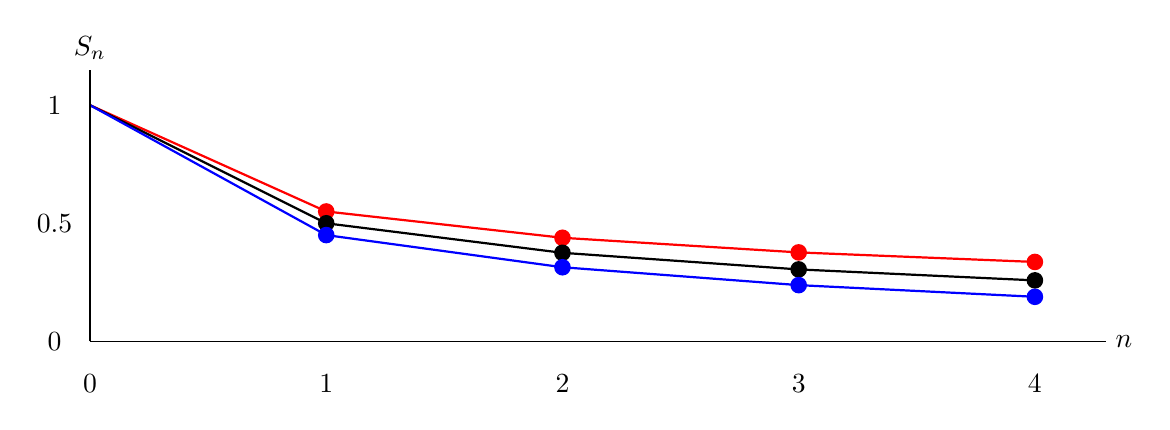
\begin{tikzpicture}[scale = 3]
    % Scatter plot points
    \foreach \x/\y/\color in {1/0.55/red, 2/0.4386250/red, 3/0.3766719/red, 4/0.336304/red,
                                                1/0.5/black, 2/0.375/black, 3/0.3046875/black, 4/0.25827/black,
                                                   1/0.449999/blue, 2/0.313874/blue, 3/0.2381546/blue, 4/0.188816/blue}
      \fill[color=\color] (\x, \y) circle (1pt);

    % Trajectories
    \draw[red, thick] (0, 1) -- (1, 0.55) -- (2, 0.4386250) -- (3,0.3766719) -- (4,0.336304);
    \draw[black, thick] (0, 1)--(1,0.5) --  (2,0.375) -- (3,0.304687) -- (4,0.25827);
    \draw[blue, thick] (0, 1)--(1,0.449999)  --  (2,0.313874) -- (3,0.238154) -- (4,0.18881);

    % Axis labels
    \draw[-] (0,0) -- (4.3,0) node[right] {$n$};
    \draw[-] (0,0) -- (0,1.15) node[above] {$S_n$};

    % Time points
    \foreach \x/\label in {0/0, 1/1/, 2/2/, 3/3, 4/4}
      \node at (\x, -0.18) {\label};
      
      \foreach \y/\label in {0/0, 0.5/0.5, 1/1/}
      \node at (-0.15, \y) {\label};
  \end{tikzpicture}

\end{center}



\subsection*{An initial infectious cohort of size $k$}
Now suppose that $X_0 = k$. Instead of the process beginning with a single unit, it starts out with a group; and for the sake illustration, we can assume this bunch is small to moderate in number, perhaps around $k = 10$.\par Given we assume supercritical branching, as the bacterial count increases, the population growth will naturally become more predictably exponential in nature. A large number of cohort units causing the expected dynamics to shine through, emergent from the haze of individual stochasticity.\par


And so, for or this initial colony --- maybe $k = 10$ pathogenic bacteria in a mammalian host --- what are its chances of persistence? Of going on to found a full blown infection?  \par
We can address this question by considering the probability with time that at least one descendent remains from the first colony. This is the likelihood that not every lineage has gone extinct. Given a single lineage dies out with the above described probability, ${}_1u_n$, the chance of all $k$ lineages dissapearing is $\lrb{{}_1u_n}^k$. Hence the probability of population persistence, in at least some descendant, is 
$$S^{(k)}_n = 1 - \lrb{{}_1u_n}^k.$$


\begin{figure}
\centering
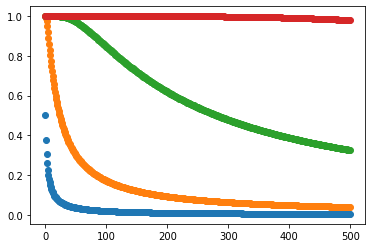
\includegraphics[width=0.6\textwidth]{figures/IMG_ch3/kvals.png}
\caption{Survival probability out to 500 generations with 1, 10, 100, and 1000 initial individuals. (From blue to red).  }
\label{fig1}
\end{figure}

\noindent
Figures \ref{fig1} and \ref{fig2} show the values of $S_n^{(k)}$ through 500 generation for $k$ = 11, 10, 100, and 1000. The effect seen in figure \ref{fig1}, that a greater first cohort gives improved longevity, is highly sensitive to the criticality of the process. So persistence develops quickly as $p$ approaches 0.5 from below, and it continues to improve dramatically into supercriticality. To illustrate this, figure \ref{fig2} shows the same experiment done with $p$ slightly above and below 0.5. 



\begin{figure}
\centering

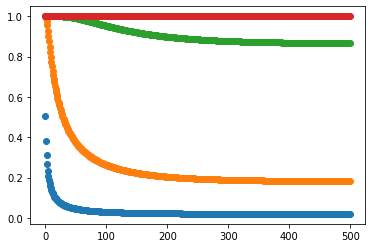
\includegraphics[width=0.45\textwidth]{figures/IMG_ch3/kvals505.png}
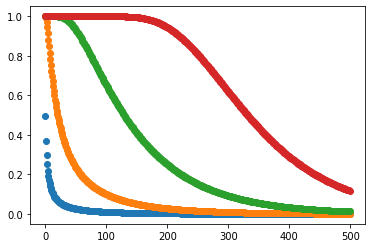
\includegraphics[width=0.45\textwidth]{figures/IMG_ch3/kvals495.png}
\caption{Like figure \ref{fig1} but the value of $p$ is no longer exactly critical at 0.5. On the left, it is supercritical at 0.505; for the right, 0.495. }
\label{fig2}
\end{figure}

\subsection*{Potential implications}

Firstly, it seems if nothing else a curiosity, that this observation aligns with a point made be R. Mann in a recent paper on modelling the longevity and size of phylogenetic clades. Here it was highlighted that those clades which have persisted through the ages, and are often of superior diversity, happened to have experienced an above average early rate of species origination. As far as I understand, this is an observation from the fossil record itself. Mann et al. argued that this empirical fact can be explained merely as a statistical consequence. As, if you were to run, as they did, a large number of homogeneous birth death processes, and select only those which happen to survive to some arbitrary large positive time ---  ``the present''. 



A hypothesis: It is of pathogenic advantage for an agent to ensure a high security of early initial replication, even at some cost to individual unit survival through later generations. 


\subsection{Discrete Birth-death-catastrophe --- does it have a stationary limiting distribution?}

Until the point of catastrophe, a discrete time BDC process will exhibit the same behaviour with regards to its stationary conditional limiting distribution as the basic Galton Watson model. \par
So conditioning on non-rupture, the process, when also conditioned on non extinction by death, exhibits a stationary limiting distribution. Does this mean that there will be a quasi-stationary distribution when conditioning on neither death nor catastrophe. In any case, we can test this with simulations.\par
But in addition, it will prove helpful to figure out some probability of non-catastrophe with advancing generations.
\subsection*{Probability of rupture at step $n$}

If the probability that a given individual will initiate catastrophe is $k$, the we can specify the probability that none of a size $N$ cohort will do so at an iterative step. A single individual will not cause rupture with probability $1-k$, two wp $(1-k)^2$, three, $(1-k)^3$, so on and so forth... \par
Considering for now the case of only birth and catastrophe --- no death --- it can be said with certainty the census of a living population at arbitrary generation, $n$. With a single progenitor, it is simply the case that the population will double at each step prior to catastrophe. Hence, the process will come to its abrupt halt in generation $n$ with probability
$$1-(1-k)^{2^{n-1}}$$
(not every individual didn't cause catastrophe).

\subsection*{Probability of process survival}
Thinking along these lines we can define (for the no death case)  the probability that a process survives to generation $n$. Lets call it $S_n$. For generation 0, this is clearly certain ($S_0=1$). Survival to generation one simply requires that the first individual replicated, $S_1 = (1-k)$. For persistence to step 2, not only must the first unit divide, but so must each of its offspring: $$S_2 = (1-k)(1-k)^2.$$ And so a pattern can be seen. For survival to the $n$th generation, every step prior must have been passed. Hence,
$$S_n = \Pi_{i = 0}^{n-1} (1-k)^{2^i} = (1-k)^{\sum^{n-1}_{i=0}2^i}.$$

\subsection*{Death included}
The difficulty comes in defining $S_n$ when death is allowed. In this version, the size of a living population can no longer be known with certainty through the generations. The question I would now like to address, is do the probabilities some how ``shake out'' when the expected value of the process is used; is the following correct? 
$$S_n  = (1-k)^{\sum^{n-1}_{i=0}\mean{\xx_i}}.$$
I suspect it isn't. But probably worth checking. 


\subsection{Continuous time birth death --- Survival probability and QS distribution}


From Linda Allen's book, we have the probability of extinction for the simple birth death process: 
$$p_0(t) = \begin{cases}
\lrb{\frac{\mu - \mu e^{(\mu - \lambda) t }}{  \lambda  - \mu e^{(\mu - \lambda) t }}}^N, \;\; &\lambda \neq \mu\\ 
\lrb{\frac{\lambda t}{1 + \lambda t}}^N, \;\;& \lambda = \mu.
\end{cases}$$
From this, we also have the probability of process survival at time $t$:
$$S^{(N)}(t) = 1 - p_0(t)$$

\subsection*{Limiting mean conditioned on non-extinction}
The simple birth-death model has a stationary mean when $\mu < \lambda$. We can demonstrate this simply in the following way. The conditional mean can be obtained via,
\begin{equation}
\label{condit}
\mean{\xt | \xt > 0} = \frac{\mean{\xt} }{S^{(N)}(t)}.
\end{equation}
And the late time limit of this can be evaluated using L'hopital's rule. When $\mu < \lambda$, 
$$\lim_{t\to\infty}\mean{\xt | \xt > 0}  = \frac{\mu}{\mu - \lambda} = \frac{1}{1 - \frac{\lambda}{\mu}}$$

\subsection*{More simply}

Taking $N=1$, when $\lambda < \mu$: 
$$\mean{\xt } = \ee^{(\lambda - \mu)t}$$
and,
\begin{align*}
S(t) &= 1 - \lrb{\frac{\mu - \mu \ee^{(\mu - \lambda)t}}{\lambda - \mu \ee^{(\mu-\lambda)t}}} \\
&= \frac{\lambda - \mu}{\lambda - \mu \ee^{(\mu - \lambda)t}}.
\end{align*}
So given (\ref{condit}),
$$\mean{\xt | \xt > 0} = \frac{\lambda\ee^{(\lambda-\mu)t} - \mu}{\lambda - \mu}.$$
In the case considered, $\lambda > \mu$, the limiting conditional mean becomes a constant:
$$\lim_{t\to\infty}\mean{\xt | \xt > 0}  = \frac{\mu}{\mu - \lambda}  \lrb{ = \frac{1}{A}}$$.
This may be represented as
$$\frac{1}{A} = \frac{1}{1 - \frac{\lambda}{\mu}};$$
and writing in terms of replication probability, $p = \lambda/(\lambda + \mu)$,
$$\frac{1}{A} = \frac{1-p}{1-2p};$$
inverse of the quasi-stationary mean,
$$A = \frac{1-2p}{1-p}.$$


\begin{center}
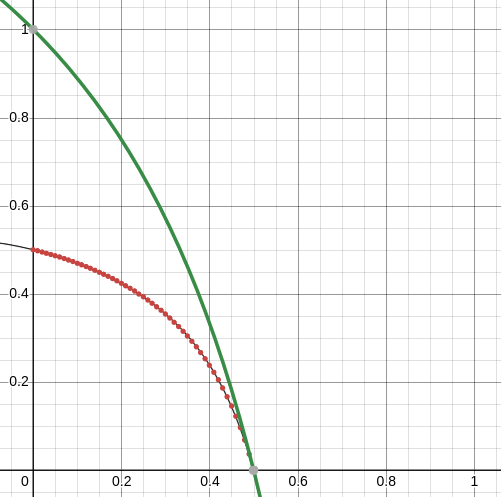
\includegraphics[width=0.45\textwidth]{figures/IMG_ch3/dtctA.png}
\end{center}

\noindent
In the figure above, the green line is $A$ as defined above. The red dots represent precise numerically obtained values of the analogous measure in the discrete time Galton Watson process; the black line is a closely matching formula found computationally \cite{cohen2024physics} \cite{stanley2002evolving}.\par
The obvious question which comes to mind is: why does the curve start at 1 in continuous time and 0.5 in discrete time. Merely dividing the ``green'' formula by 2 doesn't cause an overlap.



%%%%%%%%%%%%%%%%%%%%%%%%%%%%%%%%%%%%%%%%%%%%%%%%%%%%%%%%%%%%%%%%%%%%%%%%%%%%%%%%%%%%%%%%%%%%%%%%%%%%%%%%%% MOC
